\section{Question 4}

\begin{question}
    Considering the K-Nearest Neighbor (K-NN) classifier and performing a 10-fold Stratified
    CrossValidation, what is the impact of parameter K on the average classifier accuracy? Report at
    least 5 screenshots showing the confusion matrices achieved using different K parameter values.
\end{question}

\begin{answer}
    Figure 9 shows the impact of \textbf{k} on the model. Increasing the value, we see a significant
    improvement from 1 to 5, but after that with 10 there is no improvement. Actually it decreases
    the recall for the recurrence-events class. After that with a high value (100), the model lean
    completely to the 'no-recurrence-events' class. A good value for the model would be 5.

    \begin{figure}
        \centering
        \subfigure[]{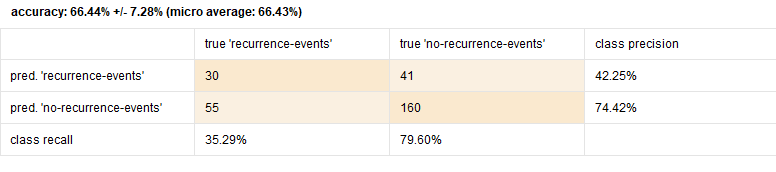
\includegraphics[width=0.48\textwidth]{Screenshot_25.png}}
        \subfigure[]{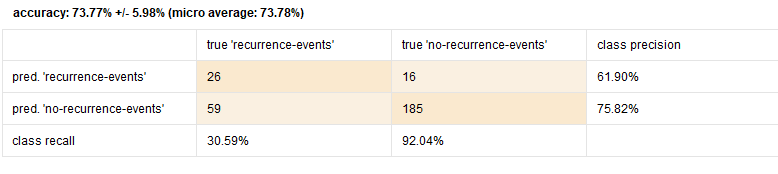
\includegraphics[width=0.48\textwidth]{Screenshot_26.png}}
        \subfigure[]{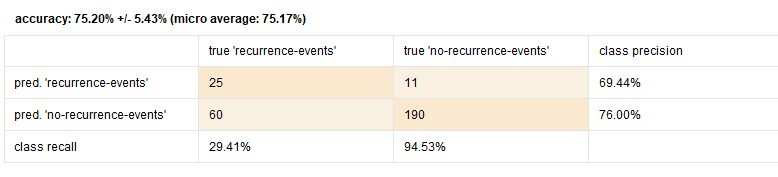
\includegraphics[width=0.48\textwidth]{Screenshot_27.png}}
        \subfigure[]{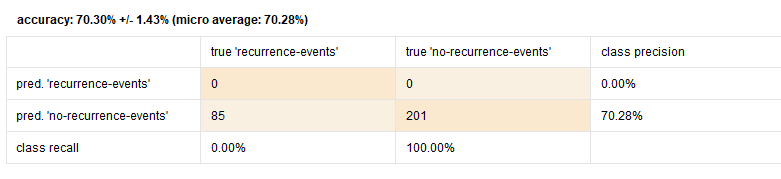
\includegraphics[width=0.48\textwidth]{Screenshot_28.png}}
        \caption{Impact of the \textbf{k} with values
            \\
            (a) 1 (b) 5 (c) 10 (d) 100}
    \end{figure}
\end{answer}

\begin{question}
    Perform a 10-fold Stratified Cross-Validation with classifier Naïve Bayes. Does K-NN perform on
    average better or worse than the Naïve Bayes classifier on the analyzed data? Report a screenshot
    showing the confusion matrix achieved by Naïve Bayes on the analyzed dataset
\end{question}

\begin{answer}
    Figure 11 shows how Naive Bayes classifier perform better than K-NN classifier. With any K value
    K-NN reaches a so good recall/precision balance for the 'recurrence-events' class. However, Naive Bayes
    classifier is not tunable, so if the Business Context require any adjustment, the Naive Bayes has that
    draw back.
    \begin{figure}
        \centering
        \subfigure[]{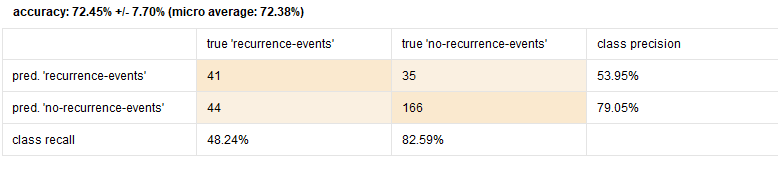
\includegraphics[width=0.48\textwidth]{Screenshot_29.png}}
        \caption{Naive Bayes classifier performance}
    \end{figure}
\end{answer}
\pagebreak